\section{Planificación}
Para tener claras las actividades a realizar, se ha realizado una planificación de las mismas, usando la herramienta Figma: 
\begin{figure}[H]
  \centering
  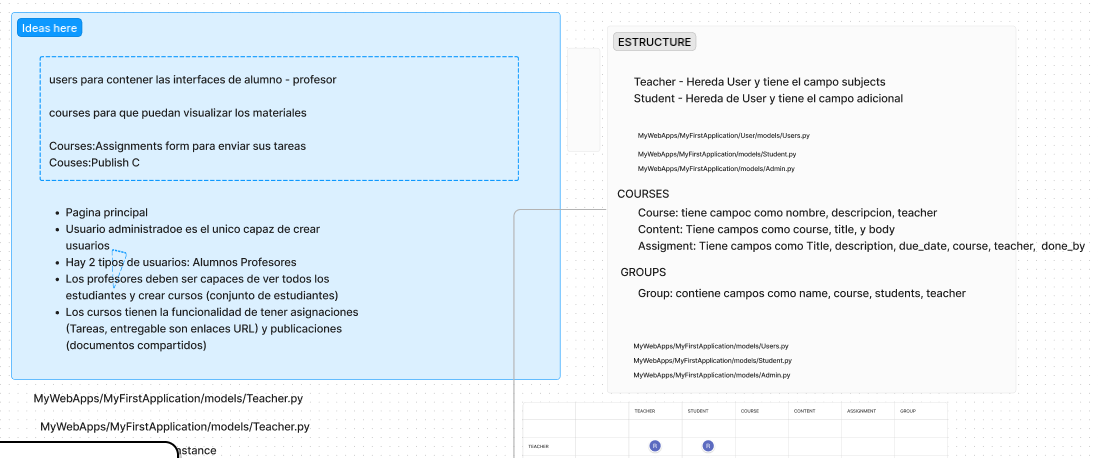
\includegraphics[width=0.8\textwidth]{img/planificacion.png}
  \caption{Planificación de actividades}
\end{figure}

\section{Modelo de datos}
Para el desarrollo de la aplicación se ha planteado el siguiente modelo de datos:
\begin{figure}[H]
  \centering
  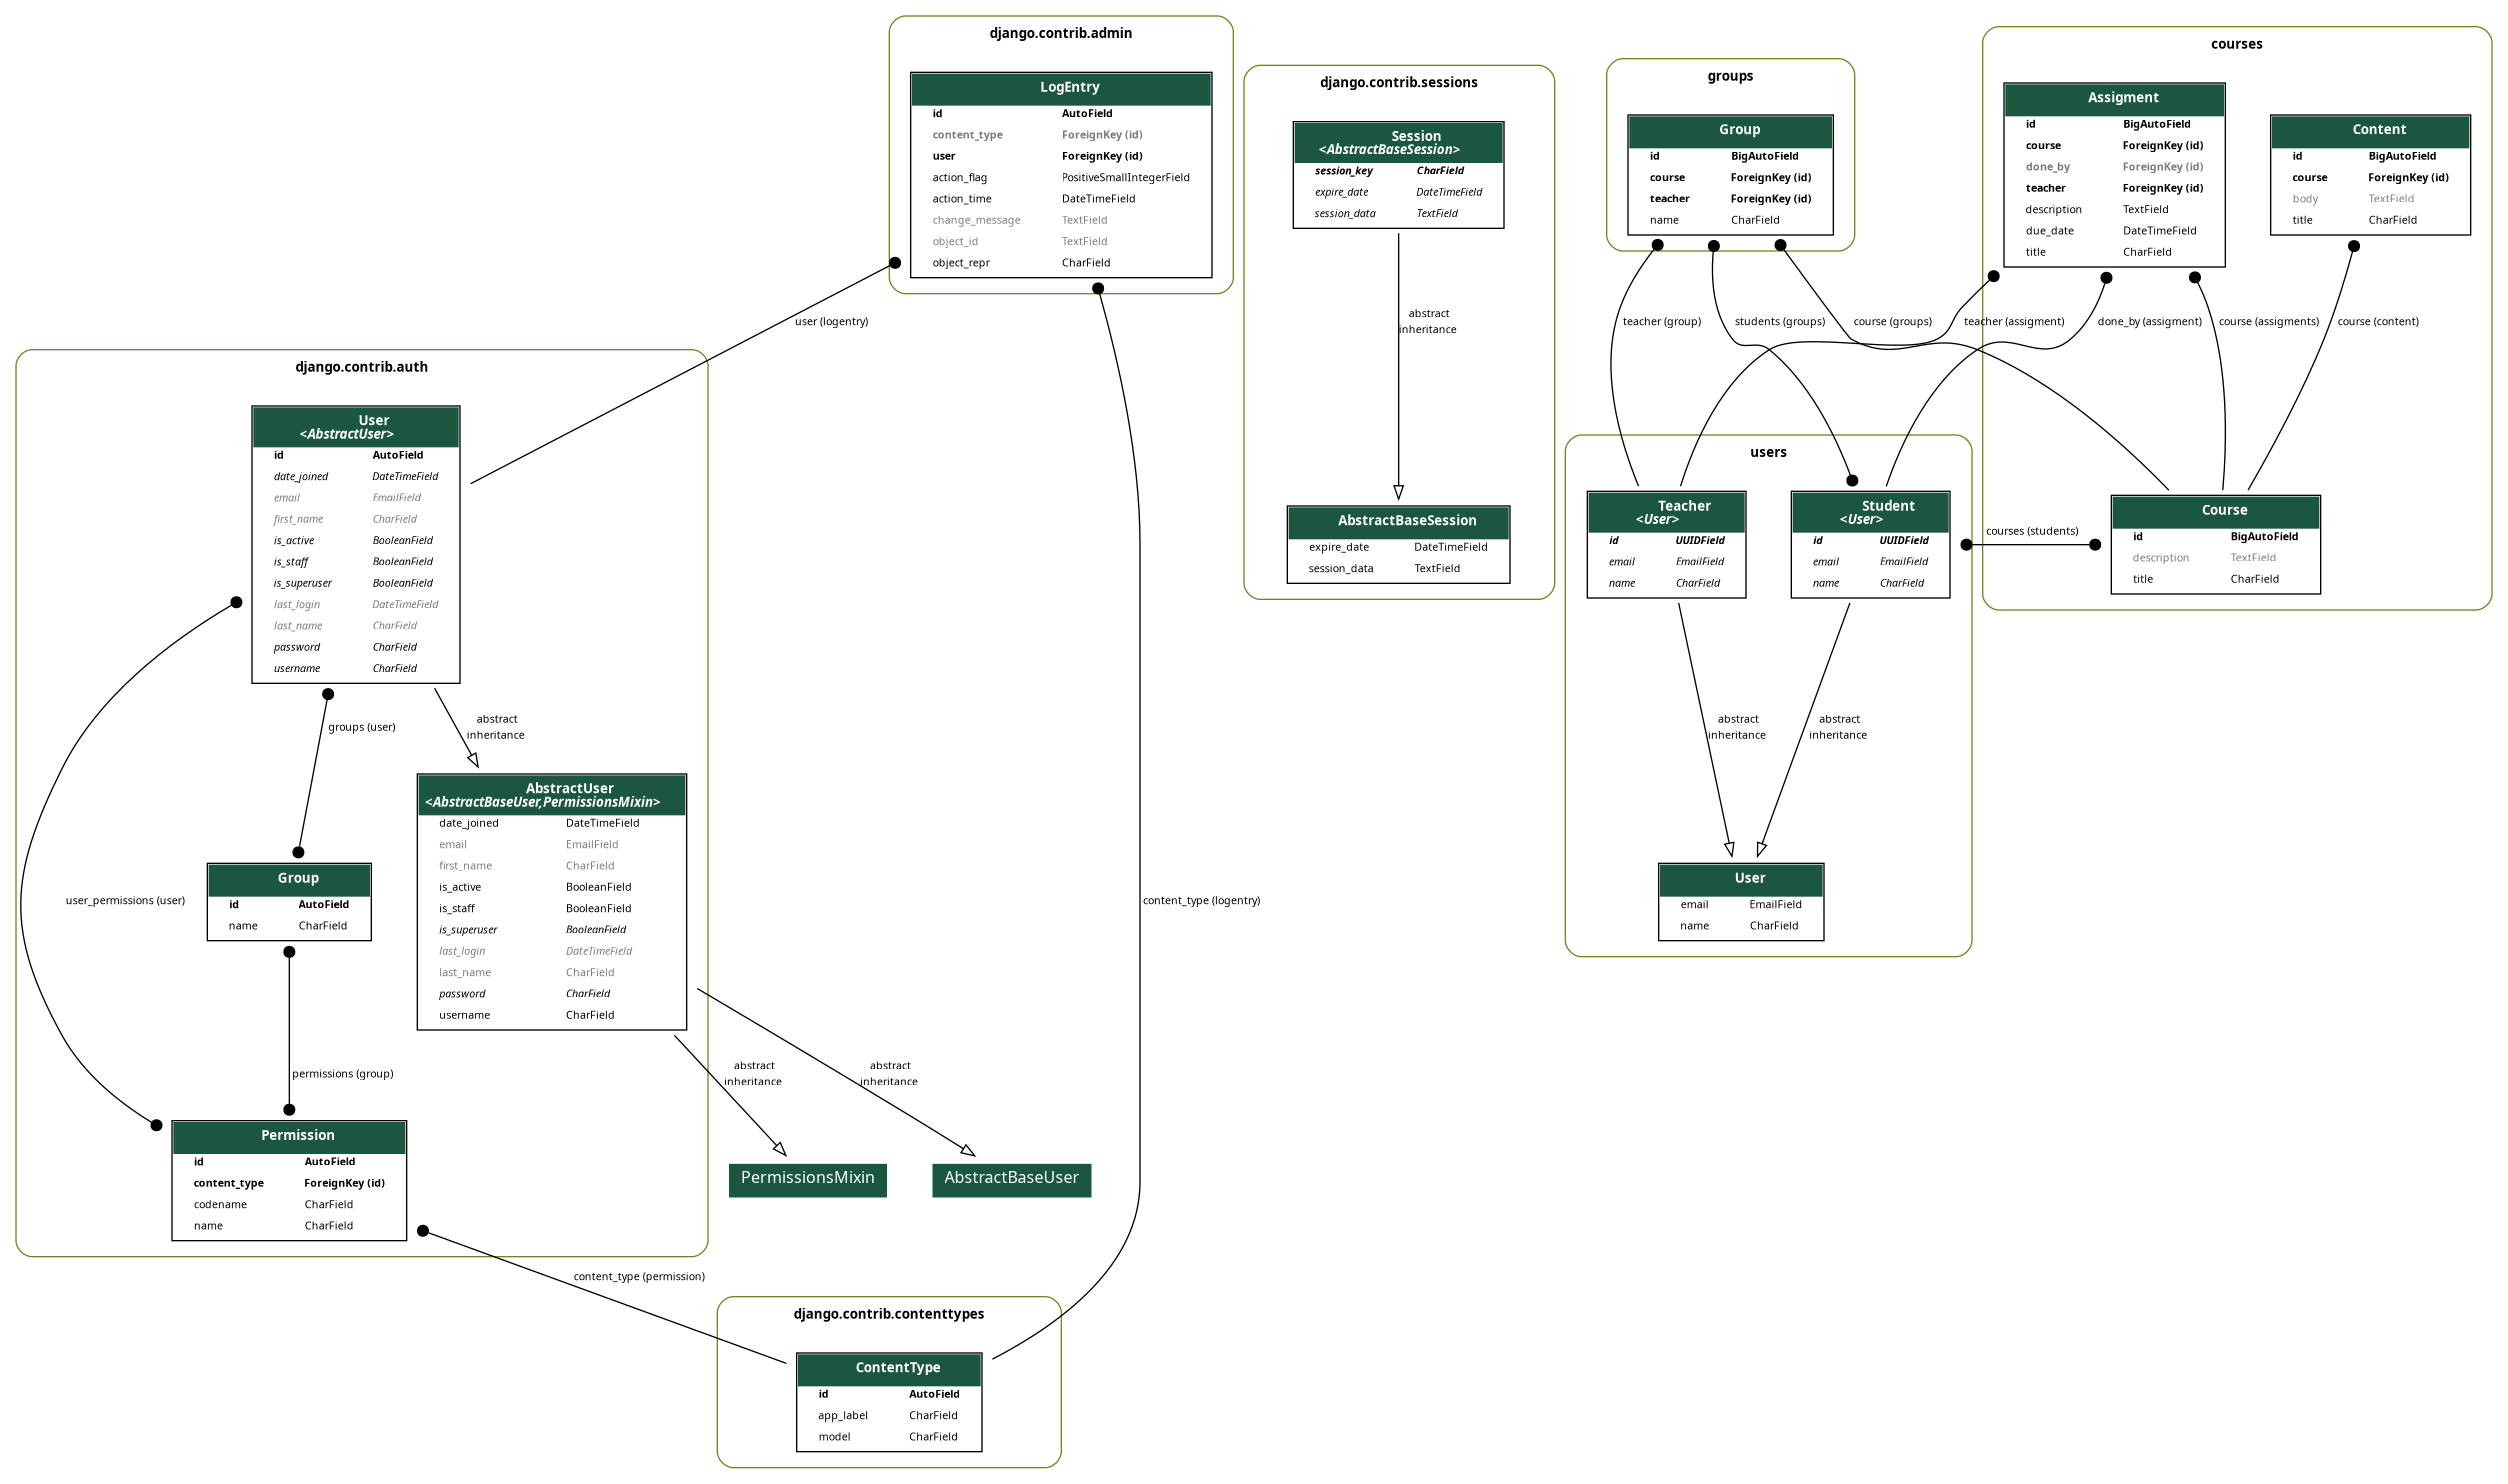
\includegraphics[width=0.8\textwidth]{img/diagrama.png}
  \caption{Modelo de datos}
\end{figure}

A continuacion veremos una explicacion mas detallada sobre los modelos en Django.

\section{Modelos Python}
Los siguientes modelos fueron creados en Django, en archivos separados, en la carpeta models de cada aplicación:

\subsection{Student}

El modelo Student hereda de User, y tiene una relación de muchos a uno con Course, es decir, un estudiante puede estar inscrito en varios cursos, pero un curso solo puede tener un estudiante.

\begin{lstlisting}[language=Python]
class Student(User):
    courses = models.ForeignKey(Course, related_name='students', on_delete=models.CASCADE)
\end{lstlisting}

\subsection{Teacher}

El modelo Teacher hereda de User, y tiene una relación de muchos a uno con Groups, que maneja la lógica de los grupos de estudiantes y sus cursos. 

\begin{lstlisting}[language=Python]
class Teacher(User):
    pass
\end{lstlisting}

\subsection{Course}
El modelo Course tiene un título y una descripción, y una relación de muchos a uno con Teacher, es decir, un curso solo puede tener un profesor, pero un profesor puede tener varios cursos.

Los campos title y description son obligatorios, y el campo teacher es opcional.

\begin{lstlisting}[language=Python]
class Course(models.Model):
  title = models.CharField(max_length=255, blank=False, null=False)
  description = models.TextField(blank=True, null=False)

  #teacher = models.ForeignKey(Teacher, on_delete=models.CASCADE)
  def __str__(self):
    return self.title
\end{lstlisting}

\subsection{Content}

El modelo Content tiene un título y un cuerpo, y una relación de muchos a uno con Course, es decir, un contenido solo puede pertenecer a un curso, pero un curso puede tener varios contenidos.

Representa el contenido de un curso, como una lección, un video, un archivo, etc.

\begin{lstlisting}[language=Python]
class Content(models.Model):
  course = models.ForeignKey(Course, on_delete=models.CASCADE)
  title = models.CharField(blank=False, max_length=255, null=False)
  body = models.TextField(blank=True, null=False)

  class Meta:
    ordering = ['course', 'title', 'body']

  def __str__(self):
    return self.title
\end{lstlisting}

\subsection{Assigment}

El modelo Assignment tiene un título, una descripción, una fecha de entrega, y una relación de muchos a uno con Course y Teacher, y una relación de uno a uno con Student, es decir, una tarea solo puede ser asignada a un estudiante, pero un estudiante puede tener varias tareas.

Los estudiantes enviarán sus tareas a través de la aplicación, y los profesores podrán calificarlas, mediante un link.

\begin{lstlisting}[language=Python]
class Assignment(models.Model):
    title = models.CharField(max_length=255, blank=False, null=False)
    description = models.TextField(blank=False, null=False)
    due_date = models.DateTimeField()
    course = models.ForeignKey(Course, related_name='assigments', on_delete=models.CASCADE)
    teacher = models.ForeignKey('users.Teacher', on_delete=models.CASCADE)
    done_by = models.ForeignKey('users.Student', null=True, blank=True, on_delete=models.SET_NULL)

    def __str__(self):
        return self.title
  \end{lstlisting}

  \subsection{Groups}

El modelo Group tiene un nombre, una relación de muchos a uno con Course y Teacher, y una relación de muchos a muchos con Student, es decir, un grupo solo puede tener un profesor y un curso, pero un profesor puede tener varios grupos, y un grupo puede tener varios estudiantes.

Los grupos representan la división de los estudiantes en clases, y cada grupo tiene un profesor y un curso asignado.

  \begin{lstlisting}[language=Python]
class Group(models.Model):

    name = models.CharField(max_length=255, blank=False, null=False)
    course = models.ForeignKey(Course, related_name='groups', on_delete=models.CASCADE)
    students = models.ManyToManyField('users.Student', related_name='groups')
    teacher = models.ForeignKey('users.Teacher', on_delete=models.CASCADE)
    
    def __str__(self):
        return self.name
    \end{lstlisting}

